\section*{Introduction}
\addcontentsline{toc}{section}{Introduction}

Pour mener à bien le projet Numeris229, il est essentiel d'explorer les concepts théoriques, les technologies et les solutions existantes dans le domaine de l'assistance conversationnelle appliquée à l'accès au droit. Ce chapitre pose les fondements du projet. Il s'articule en quatre sections : une clarification des concepts clés mobilisés, une présentation des approches techniques existantes pour améliorer les systèmes RAG, un état de l'art contextualisant les initiatives d'IA juridique et administrative en Afrique et au Bénin, et une étude comparative de quelques plateformes représentatives du domaine.

\section{Clarification conceptuelle}

\subsection{Agent conversationnel et chatbot juridique}

Un agent conversationnel, communément appelé chatbot, est un programme informatique capable d'interagir avec un utilisateur humain en langage naturel. On distingue les agents à base de règles, dont les réponses suivent des scénarios prédéfinis, des agents à base d'apprentissage automatique, capables de générer des réponses contextuelles à partir de modèles entraînés. Dans le cadre de Numeris229, l'agent conversationnel appartient à la seconde catégorie, augmenté d'un mécanisme de récupération documentaire garantissant que chaque réponse reste ancrée dans le texte officiel du code du numérique, et non dans la connaissance générale, potentiellement erronée, du modèle de langage.

\begin{figure}[H]
\centering

\begin{subfigure}[t]{0.45\textwidth}
    \centering
    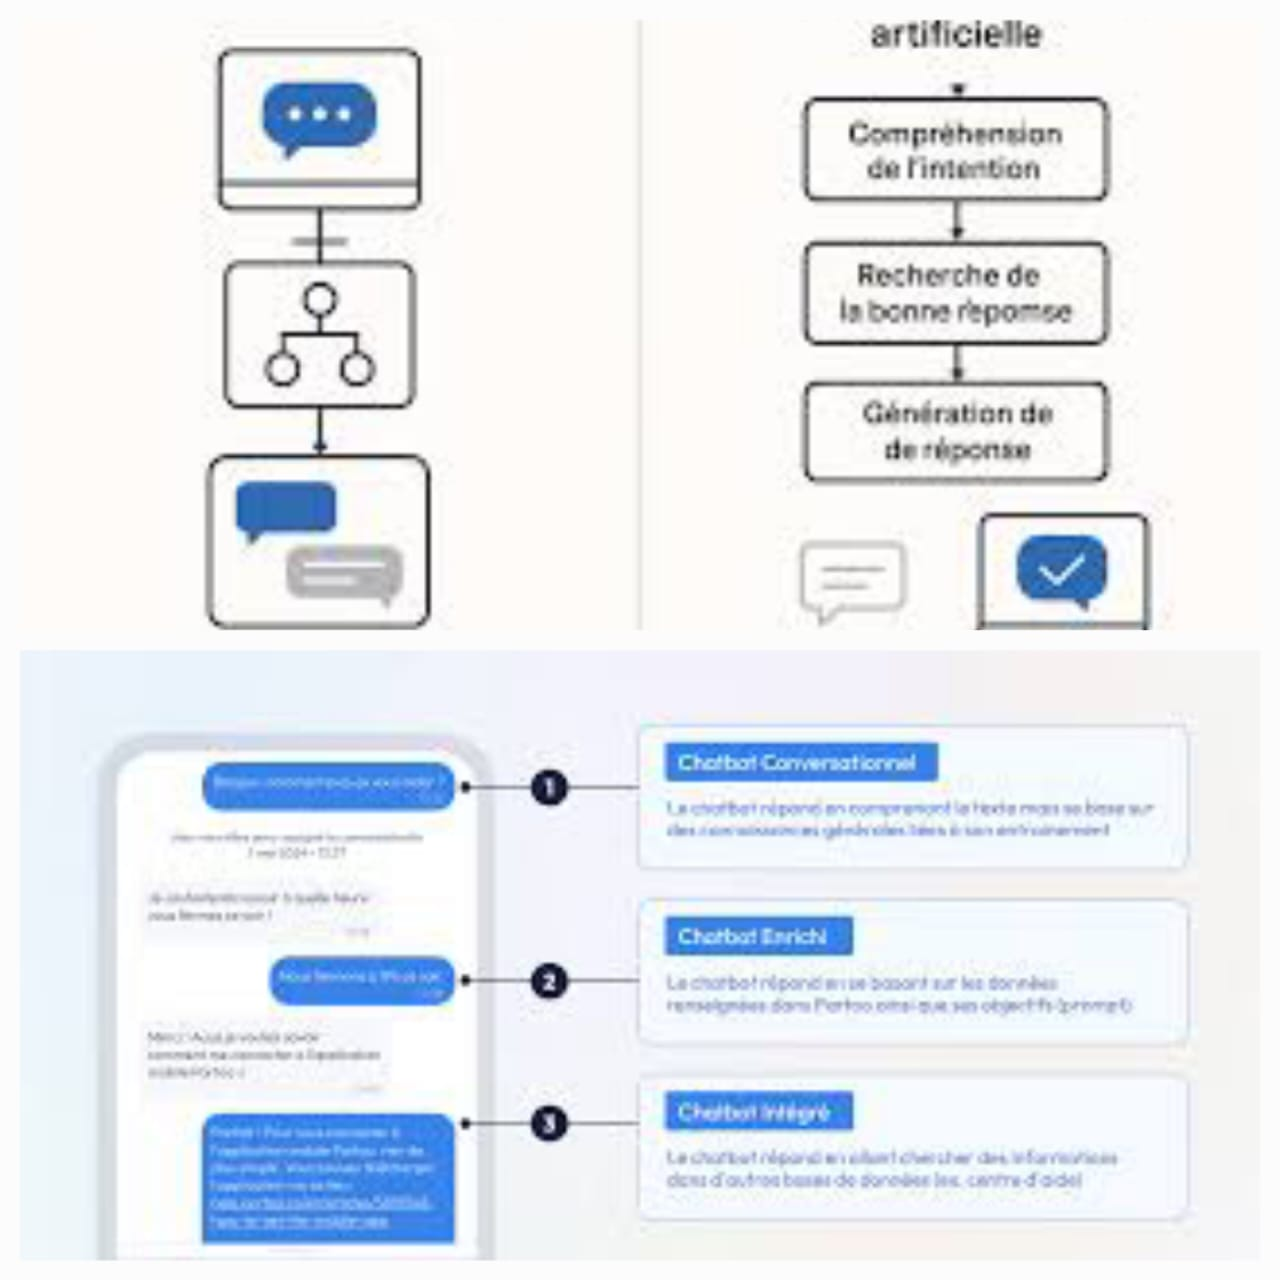
\includegraphics[width=\textwidth]{images/C1/Image2.png}
    \caption{Agent à base de règles}
\end{subfigure}
\hfill
\begin{subfigure}[t]{0.45\textwidth}
    \centering
    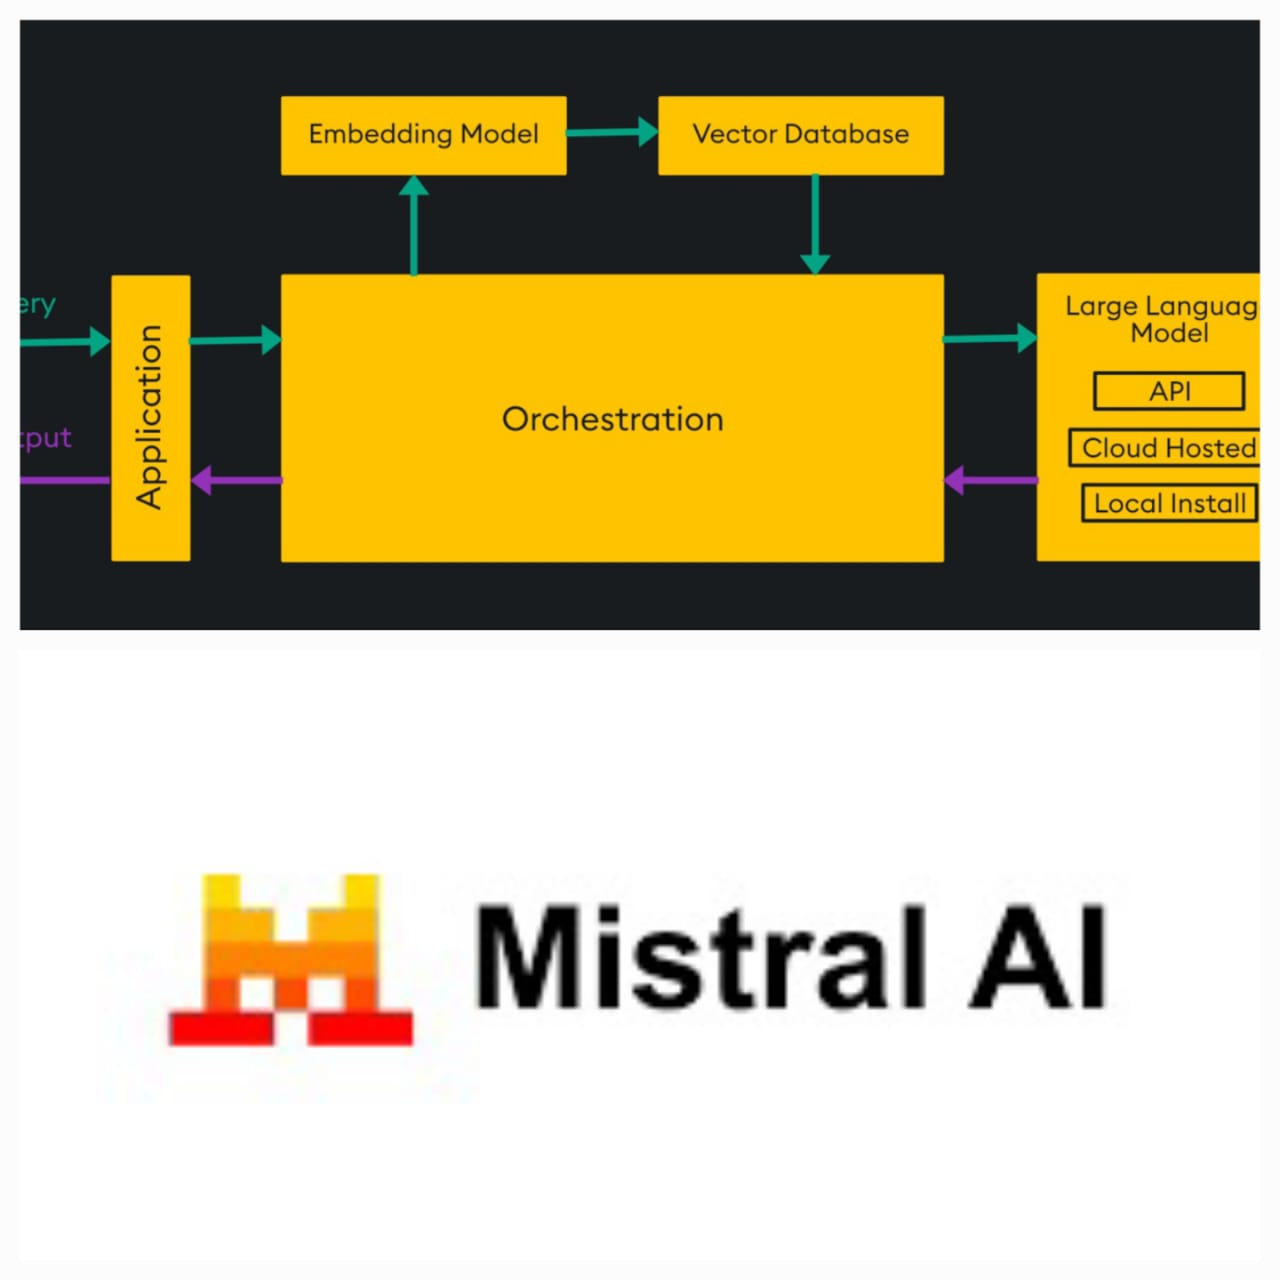
\includegraphics[width=\textwidth]{images/C1/Image1.png}
    \caption{Agent basé sur l’apprentissage automatique}
\end{subfigure}

\caption{Les deux types d’agents conversationnels}
\label{fig:chatbots}
\end{figure}

\subsection{Grands modèles de langage (LLM) et hallucination}

Les grands modèles de langage (LLM) sont des modèles d'apprentissage profond entraînés sur d'importants volumes de texte, capables de comprendre et de générer du langage naturel pour accomplir des tâches variées. Leur principale limite réside dans le phénomène d'hallucination : en l'absence d'ancrage documentaire, un LLM peut produire une affirmation plausible mais factuellement incorrecte. Ce risque est particulièrement critique dans un contexte juridique, où une référence erronée à un article de loi peut induire l'utilisateur en erreur sur ses droits ou ses obligations.

\begin{figure}[H]
\centering
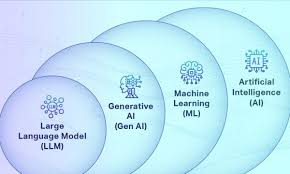
\includegraphics[width=0.6\textwidth]{images/C1/IAG LLM.png}
\caption{IAG et LLM}
\label{fig:chatbot_regle}
\end{figure}

\subsection{Architecture RAG (Retrieval-Augmented Generation)}

L'architecture RAG désigne une approche hybride combinant un module de récupération, qui extrait à partir d'une requête les passages les plus pertinents d'une base documentaire, et un module de génération, qui utilise ces passages comme contexte pour produire une réponse fondée. Pour une question donnée, le système récupère un ensemble de documents maximisant un score de similarité sémantique, puis génère une réponse conditionnée à la fois par la question et par les passages récupérés. Cette architecture garantit que les réponses restent ancrées dans un corpus contrôlé et vérifiable. Dans Numeris229, le corpus est constitué du texte consolidé du code du numérique (loi n° 2017-20 du 20 avril 2018, modifiée par la loi n° 2020-35 du 06 janvier 2021), découpé en 629 articles.

\begin{figure}[H]
\centering
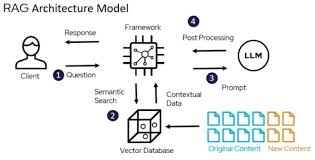
\includegraphics[width=0.6\textwidth]{images/C1/RAG.png}
\caption{RAG}
\label{fig:chatbot_regle}
\end{figure}

\subsection{Embedding et similarité sémantique}

Un embedding est une représentation vectorielle dense d'un texte dans un espace de grande dimension, telle que deux textes sémantiquement proches se trouvent à faible distance l'un de l'autre. La similarité cosinus est la mesure standard utilisée pour comparer ces vecteurs : une valeur proche de 1 indique une forte proximité sémantique. Dans Numeris229, chaque article de loi est transformé en vecteur par le modèle Solon-embeddings-base-0.1, optimisé pour la langue française, et la recherche d'un article pertinent revient à retrouver le vecteur le plus proche de la question posée par l'utilisateur.

\begin{figure}[H]
\centering

\begin{subfigure}[t]{0.45\textwidth}
    \centering
    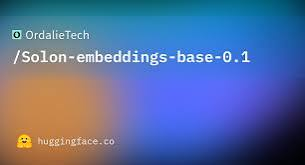
\includegraphics[width=\textwidth]{images/C1/SEB.jpg}
    \caption{Modéle Solon-embeddings-base-0.1}
\end{subfigure}
\hfill
\begin{subfigure}[t]{0.45\textwidth}
    \centering
    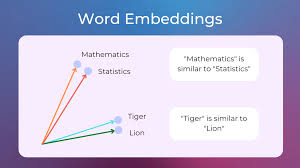
\includegraphics[width=\textwidth]{images/C1/Embedding.png}
    \caption{Embedding avec similarité sémantique}
\end{subfigure}

\caption{Le modèle d'embedding de Mistral et celui avec la similarité sémantique}
\label{fig:chatbots}
\end{figure}

\subsection{Reclassement (reranking)}

Après la phase initiale de récupération, un reranker peut être inséré pour affiner l'ordre des documents selon leur pertinence réelle par rapport à la requête, en s'appuyant sur une architecture de cross-attention qui compare finement la question et chaque passage. Cette étape réduit le bruit transmis au module de génération et améliore la précision des réponses produites.

\begin{figure}[H]
    \centering
    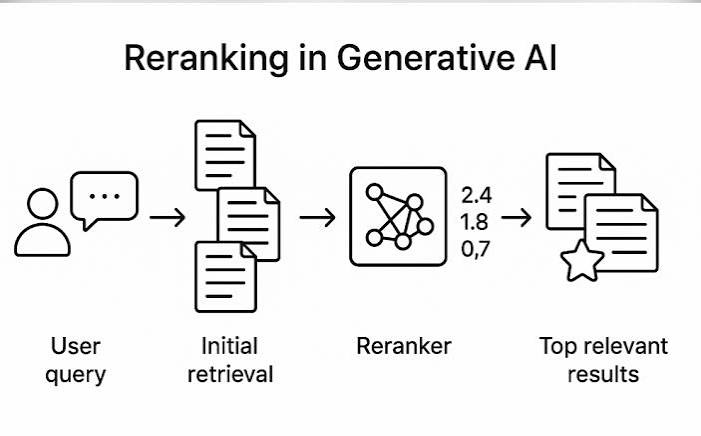
\includegraphics[width=0.45\textwidth]{images/C1/Reranker.jpg}
    \caption{Explication du Reranking}
    \label{fig:reranking}
\end{figure}

\subsection{Droit numérique et cadre juridique béninois}

Le droit numérique désigne l'ensemble des règles encadrant les activités liées aux technologies de l'information et de la communication. En République du Bénin, ce domaine est régi par le code du numérique, qui couvre notamment les réseaux et services de communications électroniques, les services de confiance en l'économie numérique, le commerce électronique, la protection des données à caractère personnel, ainsi que la cybercriminalité et la cybersécurité. Ce texte, structuré en plusieurs livres, titres, chapitres et sections, fait l'objet de modifications ponctuelles par des lois ultérieures, ce qui impose de disposer d'une version consolidée et à jour pour toute exploitation fiable.

\section{Approches techniques d'amélioration des systèmes RAG}

\subsection{Recherche hybride (Hybrid Retrieval)}

La recherche hybride s'impose comme une architecture de référence pour pallier les limites des méthodes de recherche classiques. En combinant la puissance sémantique de la recherche vectorielle avec la précision lexicale de la recherche par mots-clés, elle permet de capturer à la fois le contexte et les termes techniques spécifiques, notamment les numéros d'articles ou les intitulés précis d'une loi.

\subsection{Reclassement des documents récupérés}

Le reclassement des documents extraits par le module de récupération, en fonction d'un score de pertinence plus fin, permet de prioriser les passages réellement utiles avant leur transmission au modèle de génération, réduisant ainsi le risque d'hallucination lié à un contexte bruité.

\subsection{Recherche directe par référence structurée}

Dans un corpus juridique structuré par article, une question mentionnant explicitement un numéro d'article ne bénéficie pas toujours d'une recherche sémantique fiable, le numéro seul portant peu de signal sémantique. Une recherche directe par métadonnée structurée (numéro d'article, livre, titre, chapitre) constitue un complément nécessaire à la recherche vectorielle pour ce type de requête, préoccupation qui rejoint les enjeux d'architecture logicielle centraux à Numeris229.

\subsection{Limites de l'architecture RAG}

L'efficacité d'un système RAG dépend directement de la qualité de la requête utilisateur, de la pertinence des documents récupérés et de la fiabilité de la base de connaissances. Si cette dernière contient des documents obsolètes, non consolidés ou mal structurés, le système peut produire des réponses erronées ou trompeuses, quand bien même l'architecture de génération serait irréprochable. Cette observation justifie l'attention particulière portée, dans Numeris229, à la consolidation du corpus juridique en amont de toute indexation.

\section{État de l'art : IA conversationnelle et accès au droit en Afrique (2018--2026)}

\subsection{Chatbots juridiques généralistes}

Plusieurs chatbots destinés au grand public (Juribot, JuridiqueIA, AideJuridique.ai) proposent une assistance conversationnelle sur des questions de droit, mais restent limités au droit français et ne sont accessibles que par une interface web classique, sans canal de messagerie largement répandu dans les pays à faible connectivité.

\subsection{Plateformes juridiques pour professionnels}

Des plateformes comme Jurisprudence.cc, dédiée à l'espace OHADA, ou LawPavilion/TIMI AI au Nigeria, offrent des capacités avancées d'interrogation de bases juridiques, mais sont destinées aux avocats et magistrats, sur abonnement payant, et ne s'adressent pas au citoyen ordinaire.

\subsection{Chatbots citoyens d'accès à la justice}

Des initiatives comme Wakili.org et LegalBot au Kenya, ou JusticePadi au Nigeria, se rapprochent davantage d'un usage citoyen, intégrant parfois des langues locales. Aucune de ces solutions ne couvre cependant le cadre juridique béninois.

\subsection{Chatbots administratifs gouvernementaux}

Des assistants comme EMY 101 en Côte d'Ivoire ou GovGuideNigeria sont déployés sur des canaux de messagerie largement utilisés, mais se limitent à des démarches administratives sans couverture approfondie d'un texte de loi spécifique.

\subsection{GPT BJ : l'initiative béninoise de référence}

GPT BJ, développée par l'Agence des Systèmes d'Information et du Numérique (ASIN) avec Isheero, constitue la seule initiative d'intelligence artificielle générative souveraine documentée au Bénin. Elle compile notamment les codes des impôts, pénal, du numérique et du travail, et facilite l'accès aux réglementations nationales par le dialogue naturel. Destinée principalement à un usage gouvernemental, elle ne propose pas, à notre connaissance, de canal de messagerie grand public ni de restitution structurée article par article avec traçabilité des sources, fonctionnalités que Numeris229 place au cœur de son architecture.

\subsection{Synthèse et lacunes identifiées}

L'examen de ces initiatives révèle deux lacunes principales pour le cas spécifique du code du numérique béninois : d'une part, l'absence d'un système combinant une couverture exhaustive et à jour de ce texte (incluant ses lois modificatrices) avec une restitution sourcée au niveau de l'article ; d'autre part, l'absence d'une architecture logicielle documentée, modulaire et testable, conçue pour être maintenue et étendue dans la durée plutôt que livrée comme un prototype figé.

\section{Étude de quelques plateformes existantes}

\subsection{GPT BJ (Bénin)}

Développée par l'ASIN, GPT BJ constitue le socle d'IA générative souveraine le plus proche du contexte de Numeris229. Son architecture technique précise n'est pas publiquement documentée, mais sa couverture multi-codes et son absence de canal de messagerie grand public la distinguent d'une solution centrée sur un seul texte, avec une restitution sourcée à l'article.

\subsection{LawPavilion / TIMI AI (Nigeria)}

Cette plateforme offre une recherche avancée de jurisprudence et de textes législatifs ouest-africains, avec une architecture combinant recherche documentaire et génération assistée. Son modèle économique par abonnement et son positionnement à destination des professionnels du droit la rendent peu accessible au citoyen ordinaire, contrairement à l'objectif de Numeris229.

\begin{figure}[H]
\centering

\begin{subfigure}[t]{0.45\textwidth}
    \centering
    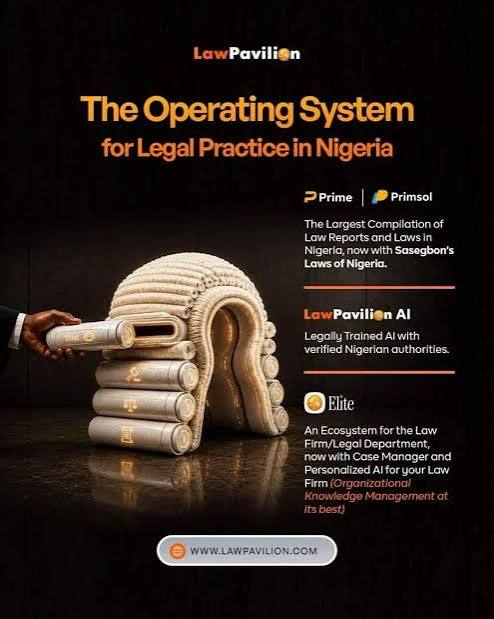
\includegraphics[width=\textwidth]{images/C1/LawPavillon.jpg}
    \caption{LawPavillon}
\end{subfigure}
\hfill
\begin{subfigure}[t]{0.45\textwidth}
    \centering
    
\includegraphics[width=\textwidth]{images/C1/Timi.jpg}
    \caption{Timi AI}
\end{subfigure}

\caption{LawPavillon/Timi AI (Nigéria)}
\label{fig:chatbots}
\end{figure}

\subsection{Wakili.org (Kenya)}

Wakili.org propose une assistance juridique citoyenne via chatbot, avec une attention portée à l'accessibilité linguistique locale. Le système reste cependant circonscrit au cadre juridique kényan et ne constitue pas une solution transposable telle quelle au contexte béninois.

\begin{figure}[H]
    \centering
    
\includegraphics[width=0.45\textwidth]{images/C1/Wakili CRM.jpg}
    \caption{Le chatbot kenyan Wakili.org}
    \label{fig:wakili}
\end{figure}

\subsection{JusticePadi (Nigeria)}

JusticePadi est un assistant conversationnel d'accès à la justice destiné aux citoyens nigérians, disponible sur plusieurs canaux. Son périmètre, centré sur le droit pénal et les droits fondamentaux, ne couvre pas le domaine du numérique.

\begin{figure}[H]
    \centering
    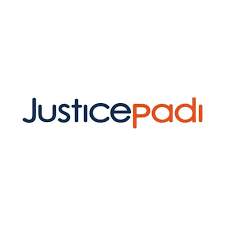
\includegraphics[width=0.45\textwidth]{images/C1/JusticePadi.png}
    \caption{Le chatbot nigérian JusticePadi}
    \label{fig:justicepadi}
\end{figure}

\subsection{EMY 101 (Côte d'Ivoire)}

EMY 101 est un chatbot administratif gouvernemental déployé sur une messagerie largement utilisée, facilitant l'accès à des démarches administratives courantes. Son architecture illustre la faisabilité technique d'un assistant accessible à grande échelle, mais sans ancrage sur un texte de loi structuré et consolidé.


\begin{figure}[H]
\centering

\begin{subfigure}[t]{0.45\textwidth}
    \centering
    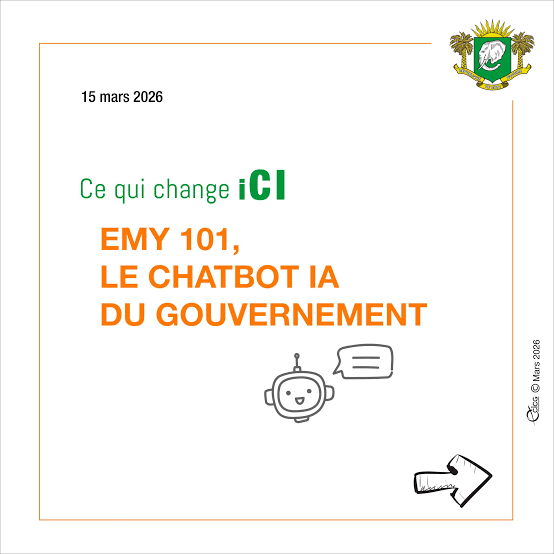
\includegraphics[width=\textwidth]{images/C1/EMY1.png}
    \caption{EMY1}
\end{subfigure}
\hfill
\begin{subfigure}[t]{0.45\textwidth}
    \centering
    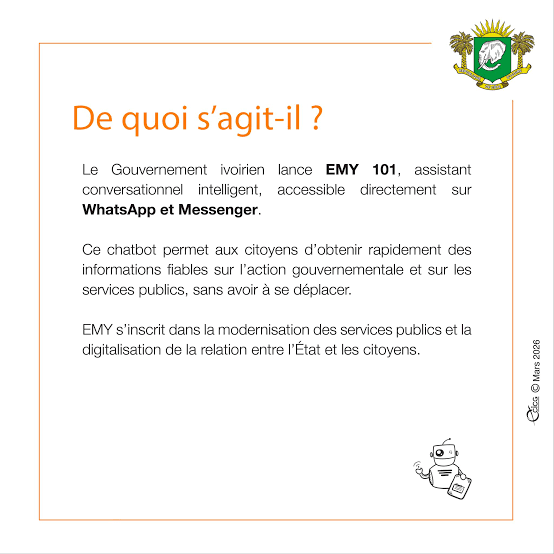
\includegraphics[width=\textwidth]{images/C1/EMY2.png}
    \caption{EMY2}
\end{subfigure}

\caption{Le chatbot EMY 101 de la Côte d'Ivoire}
\label{fig:chatbots}
\end{figure}



\section{Positionnement de Numeris229}

Par rapport aux solutions existantes, Numeris229 se distingue sur plusieurs points. D'abord, par son ancrage documentaire exclusif et consolidé sur le code du numérique béninois, incluant la prise en compte de ses lois modificatrices, ce qui garantit une réponse à jour plutôt qu'une référence à un texte obsolète. Ensuite, par une restitution systématiquement sourcée au niveau de l'article, permettant à l'utilisateur de vérifier l'information à sa source. Enfin, et surtout, par son positionnement affirmé en ingénierie logicielle : au-delà de la seule performance du modèle d'intelligence artificielle, Numeris229 propose une architecture modulaire, sécurisée et testée, de l'ingestion documentaire à la restitution finale, répondant ainsi à la lacune d'architecture logicielle documentée identifiée dans l'écosystème étudié.

\clearpage
\section*{Conclusion}
Ce chapitre a permis de présenter les concepts fondamentaux relatifs à l'intelligence artificielle conversationnelle, à l'architecture RAG et à ses techniques d'amélioration, ainsi qu'au cadre juridique du code du numérique béninois. L'étude des solutions existantes a mis en évidence l'intérêt de ces technologies pour l'accès au droit, tout en révélant l'absence d'une solution combinant couverture consolidée du code du numérique, restitution sourcée à l'article et architecture logicielle robuste et documentée. Cette situation justifie le développement de Numeris229. Les résultats de cette étude constituent une base solide pour la conception de la solution présentée dans le chapitre suivant.

\addcontentsline{toc}{section}{Conclusion}